\section{Sessão}\label{sec}

%\IEEEPARstart{E}{ste}	%Inicio de paragrafo segundo IEEE
\lipsum[1-2]		%enchedor de linguiça em latin

%\IEEEPARstart{I}{nicio}	%Inicio de paragrafo segundo IEEE
Assim\cite{python}
\gls{plugin}	%uso do glossario
\cite{thepdf}
\lipsum[3]		%enchedor de linguiça em latin, apenas paragrafo 3

% \clearpage %Forçar nova página, mesmo que \newpage
\section{Nova sessão} % (fold)
\label{sec:nova_sess_o}

\lipsum[2]		%enchedor de linguiça em latin, apenas paragrafo 2

\end{multicols}
\lstinputlisting[ %
	language=Tex, %
	caption={Exemplo de código}] %
	{./conteudo/conteudo.tex}
\begin{multicols}{2}

\lipsum[3-6]		%enchedor de linguiça em latin, apenas paragrafo 4 e 5

\end{multicols}
\begin{usecase}
    \addtitle{Caso de Uso 1}{Exemplo de caso de uso}

    \addfield{Resumo:}{\lipsum[1]}

    \addfield{Ator Primario:}{Manolo}

    \addfield{Pré-condições:}{Aplicativo instalado}
\end{usecase}
\begin{multicols}{2}

\lipsum

\end{multicols}
\begin{figure}[h]
  \begin{center}
    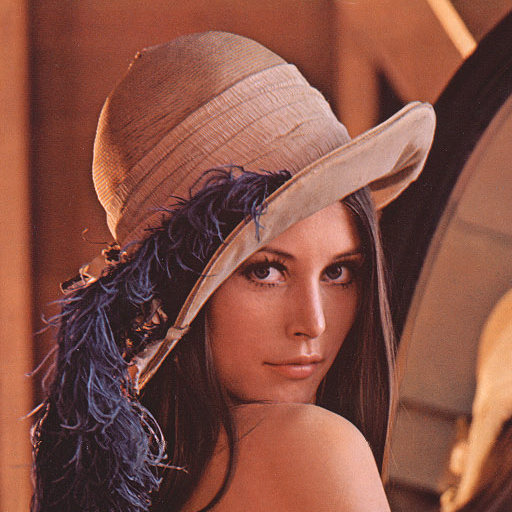
\includegraphics[width=0.8\textwidth]{conteudo/lena}
    \caption{Clássica Lena}
  \end{center}
\end{figure}
\begin{multicols}{2}

\lipsum[6]
